\documentclass[handout]{beamer}
%\documentclass[UTF8]{ctexart}
\usepackage{ctex}
\usepackage{graphicx} %插入图片用
 % 1. packages

 % ----------- fonts and symbles ---------
\usepackage{amsmath,amssymb,amsfonts,amsthm}
%\usepackage{CJK}
\usepackage{dsfont}
\usepackage{mathrsfs}
\usepackage{eucal} % for \mathcal

%\renewcommand{\rmdefault}{ptm}


%\usepackage{fontspec}
%\newfontfamily\monaco{Monaco}

%\usepackage{mathbbold} %,bbold

 \usepackage{textcomp} % for \textnormal{\textperthousand}
% -----------------





%\usepackage{slashbox}
%\usepackage[margin=2.2cm]{geometry} % |geometry| package clash with |booktabs| package
%\usepackage{cases}
% -------- tables -------
\usepackage{booktabs} % for \toprule, \bottomrule
\usepackage{tabularx}
\usepackage{multirow}
% --------- figures ---------
\usepackage{graphicx}
% ---------- algorithms -------
\usepackage{algorithm}
\usepackage{algorithmic}
%\usepackage{footnote}
    % |footnote| package occurs error:
    % Runaway argument?
    % \def \insertfootnotetext {\@@ }\def \insertfootnotemark {\@makefnmark \ETC.

\usepackage{listings}

\usepackage[linewidth=1pt]{mdframed} % for  mdframe environment




 \usepackage{color}
 \usepackage{xcolor}     %¸ßÁÁʹÓõÄÑÕÉ«

\usepackage{setspace}
%%\usepackage{type1cm}
\usepackage{adjustbox} % for \adjustbox

\usepackage{accsupp}
\newcommand{\emptyaccsupp}[1]{\BeginAccSupp{ActualText={}}#1\EndAccSupp{}}




%%   figures and tables
\graphicspath{{figure/}}


% 2. new commands

% 2.0 common commands
%\newcommand{\bc}{\begin{center}}
%\newcommand{\ec}{\end{center}}
%\newcommand{\ba}{\begin{array}}
%\newcommand{\ea}{\end{array}}
%\newcommand{\be}{\begin{equation}}
%\newcommand{\ee}{\end{equation}}

% 2.1 colors
\definecolor{dgrey}{rgb}{0.30,0.30,0.30}
\definecolor{lred}{rgb}{0.50,0.00,0.50}
\definecolor{lblue}{rgb}{0.8,0.8,1}
\definecolor{dred}{rgb}{0.6,0,0}
\definecolor{dblue}{rgb}{0,0,0.5}
\definecolor{dgrey}{rgb}{0.35,0.35,0.35}
\definecolor{rred}{rgb}{0.9,0,0}
\definecolor{mylblue}{rgb}{0.3,0.2, 0.8}

\definecolor{commentcolor}{RGB}{85,139,78}
\definecolor{stringcolor}{RGB}{206,145,108}
\definecolor{keywordcolor}{RGB}{34,34,250}
\definecolor{backcolor}{RGB}{220,220,220}

\newcommand{\blue}[1]{{\color{blue}#1}}
\newcommand{\dblue}[1]{{\color{dblue}#1} }
\newcommand{\red}[1]{{\color{red}#1}}
\newcommand{\dred}[1]{{\color{dred}#1}}
\newcommand{\cyan}[1]{{\color{cyan}#1}}
\newcommand{\bfblue}[1]{\textbf{\color{dblue}#1} }
\newcommand{\bfred}[1]{\textbf{\color{dred}#1} }
\newcommand{\green}[1]{{\color{green}#1}}
%\newcommand{\alert}[1]{{\color{red}#1}}
\newcommand{\black}[1]{{\color{black}#1}}
\newcommand{\light}[1]{{\color{blue}\textbf{#1}}}
\newcommand{\hot}[1]{{\color{dred}#1}}
 \newcommand{\highlight}[1]{ \textbf{\color{mylblue}#1}}
 \newcommand{\important}[1]{{\color{red}#1}} % for highlighting  some words

 \newcommand{\mystar}{\dred{$^{\clubsuit}$ }}
  \newcommand{\doublestar}{\dred{$^{\clubsuit\clubsuit}$ }}

\newcommand{\mynote}[1]{{\footnotesize \color{mylblue}#1}}

 \newcommand{\hint}[1]{{\small \color{mylblue}#1}}
\newcommand{\smallhint}[1]{{\small \color{dgrey}#1}}
\newcommand{\footnotehint}[1]{{\footnotesize \color{dgrey}#1}}
\newcommand{\tinyhint}[1]{{\tiny \color{dgrey}#1}}
\newcommand{\mytitle}[1]{\medskip{\large \textbf{\color{mylblue}#1}}}
\newcommand{\normaltitle}[1]{\medskip{ \textbf{\color{mylblue}#1}}}

%\newcommand{\head}[1]{\textbf{\large\color{blue}#1}}
%\newcommand{\heading}[1]{\textbf{\large\color{blue}#1}}

\newcommand{\myfbox}[2]{ \bigskip \begin{center} \fbox{\parbox{#1}{ #2  }} \end{center}\bigskip }

\newcommand{\myvar}[1]{}
%\newcommand{\mynote}[1]{#1}

% 2.2 mathematical symbols

\newcommand{\drightarrow}{\stackrel{d.}{\rightarrow}}
\newcommand{\prightarrow}{\stackrel{p.}{\rightarrow}}
\newcommand{\bernoulli}{\textnormal{Ber}}
\newcommand{\cov}{\mathsf{Cov}}
\newcommand{\corr}{\mathbf{Corr}}
\newcommand{\regret}{\textnormal{Regret}}
\newcommand{\conv}{\textnormal{conv}}
\newcommand{\dotdiv}{\stackrel{\centerdot}{-}}
\newcommand{\dom}{\textnormal{dom}}
\newcommand{\convergenceinprob}{\stackrel{P}{\rightarrow}}
\newcommand{\convergenceindist}{\rightsquigarrow}
\newcommand{\probability}{\mathbb{P}}
\newcommand{\expectation}{\mathbb{E}}
\newcommand{\epi}{\textnormal{epi}}
\newcommand{\variance}{\mathbb{V}}
\newcommand{\var}[1]{\mathbb{V}(#1)}
\newcommand{\covariance}{\mathsf{Cov}}
\newcommand{\empiricalrisk}[1]{\hat{R}(#1)}
\newcommand{\expectedrisk}[1]{R(#1)}
\newcommand{\mgf}[1]{\psi_{#1}(\lambda)}
\newcommand{\mgfexpansion}[1]{\expectation[e^{\lambda#1}]}
\newcommand{\mgfmultivariate}[1]{\expectation[e^{\lambda^\transpose#1}]}
\newcommand{\transpose}{{\mathsf{T}}}
\newcommand{\real}{\mathbb{R}}
\newcommand{\gaussian}[2]{\mathcal{N}(#1,#2)}
\newcommand{\subGaussian}[1]{\mathsf{subG}(#1)}
\newcommand{\indicator}[1]{\mathbb{I}[#1]}
\newcommand{\x}[1]{x^{(#1)}}
\newcommand{\y}[1]{y^{(#1)}}
\newcommand{\z}[1]{z^{(#1)}}
\newcommand{\feature}{x}
\newcommand{\response}{y}
\newcommand{\supofempiricalprocess}{\|\mathbb{P}_n-\mathbb{P}\|_{\decisionspace}}
\newcommand{\decisionspace}{\mathscr{F}}
\newcommand{\decisionfunction}{f}
\newcommand{\featurespace}{\mathcal{X}}
\newcommand{\classifierestimate}{\widehat{h}}
\newcommand{\classifiertrue}{h^\star}
\newcommand{\classifier}{h}
\newcommand{\hypothesisclass}{\mathcal{H}}
\newcommand{\dataset}{\mathcal{D}}
\newcommand{\defineas}{\stackrel{\textnormal{def}}{=}}
\newcommand{\rademachercomplexity}[1]{\mathsf{Rad}_n\left(#1\right)}
\newcommand{\loss}{\ell}
\newcommand{\composite}{\circ}
\newcommand{\convexhull}{\mathsf{conv}}
\newcommand{\norm}[2][2]{\|#2\|_{#1}}
\newcommand{\shatteringcoefficient}[2]{\mathcal{S}(#1,#2)}
\newcommand{\vcdimension}[1]{\mathsf{VC}\left(#1\right)}
\newcommand{\rank}{\mathsf{rank}}
\newcommand{\innerproduct}[2]{\left\langle #1, #2\right\rangle}
\newcommand{\modelparameter}{\theta}
\newcommand{\ball}[3][]{\mathcal{B}_{{#1}}\left(#2,#3\right)}
\newcommand{\metric}{d}
\newcommand{\coveringnumber}[4][]{N_{{#1}}\left(#2,#3,#4\right)}
\newcommand{\trace}{\textnormal{tr}}
\newcommand{\std}{\textnormal{std}}
\newcommand{\sgn}{\textnormal{sign}}
%\renewcommand{\span}{\textnormal{span}}

 % do not overwrite the existing command \span
 % as it leads to an error of
 %  "Missing # Inserted in Alignment Preamble" for ``align'' environment

\newcommand{\myspan}{\textnormal{span}}

%%%
\newcommand{\rightarrowd}{\stackrel{d}{\rightarrow}}
\newcommand{\rightarrowp}{\stackrel{p}{\rightarrow}}
\newcommand{\defeq}{ \stackrel{\textnormal{def}}{=}}
\newcommand{\proj}{ \textnormal{Proj}}
\newcommand{\dist}{\textnormal{dist}}

\newcommand{\argmax}{\textnormal{argmax}}
\newcommand{\argmin}{\textnormal{argmin}}
\newcommand{\subg}{\textnormal{subG}}


 \newcommand{\bba}{\mathbb{A}}
\newcommand{\bbb}{\mathbb{B}}
\newcommand{\bbc}{\mathbb{C}}
\newcommand{\bbd}{\mathbb{D}}
\newcommand{\bbe}{\mathbb{E}}
\newcommand{\bbf}{\mathbb{F}}
\newcommand{\bbg}{\mathbb{G}}
\newcommand{\bbh}{\mathbb{H}}
\newcommand{\bbi}{\mathbb{I}}
\newcommand{\bbj}{\mathbb{J}}
\newcommand{\bbk}{\mathbb{K}}
\newcommand{\bbl}{\mathbb{L}}
\newcommand{\bbm}{\mathbb{M}}
\newcommand{\bbn}{\mathbb{N}}
\newcommand{\bbo}{\mathbb{O}}
\newcommand{\bbp}{\mathbb{P}}
\newcommand{\bbq}{\mathbb{Q}}
\newcommand{\bbr}{\mathbb{R}}
\newcommand{\bbs}{\mathbb{S}}
\newcommand{\bbt}{\mathbb{T}}
\newcommand{\bbu}{\mathbb{U}}
\newcommand{\bbv}{\mathbb{V}}
\newcommand{\bbw}{\mathbb{W}}
\newcommand{\bbx}{\mathbb{X}}
\newcommand{\bby}{\mathbb{Y}}
\newcommand{\bbz}{\mathbb{Z}}

\newcommand{\bfa}{\mathbf{a}}
\newcommand{\bfb}{\mathbf{b}}
\newcommand{\bfc}{\mathbf{c}}
\newcommand{\bfd}{\mathbf{d}}
\newcommand{\bfe}{\mathbf{e}}
\newcommand{\bff}{\mathbf{f}}
\newcommand{\bfg}{\mathbf{g}}
\newcommand{\bfh}{\mathbf{h}}
\newcommand{\bfi}{\mathbf{i}}
\newcommand{\bfj}{\mathbf{j}}
\newcommand{\bfk}{\mathbf{k}}
\newcommand{\bfl}{\mathbf{l}}
\newcommand{\bfm}{\mathbf{m}}
\newcommand{\bfn}{\mathbf{n}}
\newcommand{\bfo}{\mathbf{o}}
\newcommand{\bfp}{\mathbf{p}}
\newcommand{\bfq}{\mathbf{q}}
\newcommand{\bfr}{\mathbf{r}}
\newcommand{\bfs}{\mathbf{s}}
\newcommand{\bft}{\mathbf{t}}
\newcommand{\bfu}{\mathbf{u}}
\newcommand{\bfv}{\mathbf{v}}
\newcommand{\bfw}{\mathbf{w}}
\newcommand{\bfx}{\mathbf{x}}
\newcommand{\bfy}{\mathbf{y}}
\newcommand{\bfz}{\mathbf{z}}

\newcommand{\bfA}{\mathbf{A}}
\newcommand{\bfB}{\mathbf{B}}
\newcommand{\bfC}{\mathbf{C}}
\newcommand{\bfD}{\mathbf{D}}
\newcommand{\bfE}{\mathbf{E}}
\newcommand{\bfF}{\mathbf{F}}
\newcommand{\bfG}{\mathbf{G}}
\newcommand{\bfH}{\mathbf{H}}
\newcommand{\bfI}{\mathbf{I}}
\newcommand{\bfJ}{\mathbf{J}}
\newcommand{\bfK}{\mathbf{K}}
\newcommand{\bfL}{\mathbf{L}}
\newcommand{\bfM}{\mathbf{M}}
\newcommand{\bfN}{\mathbf{N}}
\newcommand{\bfO}{\mathbf{O}}
\newcommand{\bfP}{\mathbf{P}}
\newcommand{\bfQ}{\mathbf{Q}}
\newcommand{\bfR}{\mathbf{R}}
\newcommand{\bfS}{\mathbf{S}}
\newcommand{\bfT}{\mathbf{T}}
\newcommand{\bfU}{\mathbf{U}}
\newcommand{\bfV}{\mathbf{V}}
\newcommand{\bfW}{\mathbf{W}}
\newcommand{\bfX}{\mathbf{X}}
\newcommand{\bfY}{\mathbf{Y}}
\newcommand{\bfZ}{\mathbf{Z}}


\newcommand{\bfSigma}{\mathbf{\Sigma}}
\newcommand{\bfrho}{\mathbf{\rho}}

\newcommand{\cala}{\mathcal{A}}
\newcommand{\calb}{\mathcal{B}}
\newcommand{\calc}{\mathcal{C}}
\newcommand{\cald}{\mathcal{D}}
\newcommand{\cale}{\mathcal{E}}
\newcommand{\calf}{\mathcal{F}}
\newcommand{\calg}{\mathcal{G}}
\newcommand{\calh}{\mathcal{H}}
\newcommand{\cali}{\mathcal{I}}
\newcommand{\calj}{\mathcal{J}}
\newcommand{\calk}{\mathcal{K}}
\newcommand{\call}{\mathcal{L}}
\newcommand{\calm}{\mathcal{M}}
\newcommand{\caln}{\mathcal{N}}
\newcommand{\calo}{\mathcal{O}}
\newcommand{\calp}{\mathcal{P}}
\newcommand{\calq}{\mathcal{Q}}
\newcommand{\calr}{\mathcal{R}}
\newcommand{\cals}{\mathcal{S}}
\newcommand{\calt}{\mathcal{T}}
\newcommand{\calu}{\mathcal{U}}
\newcommand{\calv}{\mathcal{V}}
\newcommand{\calw}{\mathcal{W}}
\newcommand{\calx}{\mathcal{X}}
\newcommand{\caly}{\mathcal{Y}}
\newcommand{\calz}{\mathcal{Z}}


% 3. theorem and environments

%\newtheorem{theorem}{Theorem}%[section]
\newtheorem{proposition}{Proposition}%[section]
%\newtheorem{property}{Property}%[section]
%\newtheorem{lemma}{Lemma}%[section]
%\newtheorem{corollary}{Corollary}%[section]
%\newtheorem{definition}{Definition}%[section]
%\newtheorem{example}{Example}%[section]
%\newtheorem{remark}{Remark}%[section]
%\newtheorem{note}{Note}%[section]
%\newtheorem{problem}{Problem}%[section]
\newtheorem{exercise}{Exercise}
%\newtheorem{assumption}{Assumption}
\newtheorem*{lemma_star}{Lemma}
\newtheorem*{theorem_star}{Theorem}

%\newenvironment{summary}[1][Summary]{\par\medskip   \color{dred}\textbf{\large#1. } }{ \medskip}
%\newenvironment{remark}[1][Remark]{\par\medskip  \begin{small} \color{dblue}\textbf{#1. } }{ \end{small}\medskip}
%\renewenvironment{proof}[1][Proof]{\noindent\textbf{#1.} }{\mbox{} \hfill{\small\textrm{$\Box$}}\vspace{1ex}}
% \newenvironment{answer}[1][Answer]{\par\medskip \color{dblue}\textbf{\large#1. }}{ \medskip}

\newenvironment{summary}[1][总结]{\par\medskip   \color{dred}\textbf{\large#1 } }{ \medskip}
\newenvironment{remark}[1][注意]{\par\medskip   \color{dblue}\textbf{\large#1 } }{ \medskip}
\newenvironment{footnoteremark}{ \color{dblue}\begin{footnotesize} }{\end{footnotesize}}
\renewenvironment{proof}[1][证明]{\noindent\textbf{#1.} }{\mbox{} \hfill{\small\textrm{$\Box$}}\vspace{1ex}}
 \newenvironment{question}[1][Q.]{\par\medskip {\color{lred}\large#1}}{ \medskip}
 \newenvironment{answer}[1][Answer]{\par\medskip \color{dblue}\textbf{\large#1 }}{ \medskip}

% 4. beamer setting




%\newtheorem{definition}{\textbf{¶¨Òå}}[section]
%\newtheorem{proposition}[definition] { \textbf{ÃüÌâ}}
%\newtheorem{lemma}[definition] { \textbf{ÒýÀí}}
%\newtheorem{theorem}[definition]{ \textbf{¶¨Àí}}
%\newtheorem{corollary}[definition] { \textbf{ÍÆÂÛ}}
%\newtheorem{remark}[definition] { \textbf{×¢}}
%\newtheorem{example}[definition] { \textbf{Àý}}

%\newcommand{\shadow}[1]{\begin{center}
%\bf{\textcolor{dblue}{\shadowbox{\parbox{3.8in}
% {\textcolor{red}
% {\vspace{1mm}#1}}}}}
%\end{center}}
%
%\newcommand{\head}[1]{\begin{center}
%\bf{\textcolor{dblue}{\shadowbox{\parbox{3.8in}
% {\textcolor{dred}
% {\vspace{1mm}#1}}}}}
%\end{center}}
%
%
%\newcommand{\heading}[1]{%
%  \begin{center}
%    \large\bf
%    \shadowbox{#1}%
%  \end{center}
%\vspace{1ex minus 1ex}}

% set  space above and below math equations in display style

\expandafter\def\expandafter\normalsize\expandafter{%
    \normalsize
    \setlength\abovedisplayskip{1.5ex}
    \setlength\belowdisplayskip{1.2ex}
    \setlength\abovedisplayshortskip{0.5ex}
    \setlength\belowdisplayshortskip{0.5ex}
}

% Ìí¼ÓÒ³Âë´úÂ룬¹È¸èÕÒµ½µÄ¡£
\addtobeamertemplate{navigation symbols}{}{%
    %\usebeamerfont{footline}%
    %\usebeamercolor[fg]{footline}%
    \setbeamercolor{footline}{fg=blue}
    \setbeamerfont{footline}{series=\bfseries}
    \hspace{1em}%
    \normalsize{\insertframenumber/\inserttotalframenumber}
}

% section numbering
\setbeamertemplate{section in toc}[sections numbered]
\setbeamertemplate{subsection in toc}[subsections numbered]



\lstset{                        %¸ßÁÁ´úÂëÉèÖÃ
%basicstyle=\small, % print whole listing small
%basicstyle=\footnotesize\sffamily, % print whole listing small
basicstyle=\footnotesize\rmfamily, % print whole listing small
%basicstyle=\rmfamily, % print whole listing small
    language=python,                    %PythonÓï·¨¸ßÁÁ
    %linewidth=0.9\linewidth,            %Áбílist¿í¶È
    %basicstyle=\ttfamily,              %ttÎÞ·¨ÏÔʾ¿Õ¸ñ
    commentstyle=\color{commentcolor},  %×¢ÊÍÑÕÉ«
    keywordstyle=\color{keywordcolor},  %¹Ø¼ü´ÊÑÕÉ«
    stringstyle=\color{stringcolor},    %×Ö·û´®ÑÕÉ«
    %showspaces=true,                   %ÏÔʾ¿Õ¸ñ
    numbers=left,                       %ÐÐÊýÏÔʾÔÚ×ó²à
    %numberstyle=\tiny\emptyaccsupp,     %ÐÐÊýÊý×Ö¸ñʽ
    numberstyle=\tiny,                  %ÐÐÊýÊý×Ö¸ñʽ
    numbersep=5pt,                      %Êý×Ö¼ä¸ô
    frame=single,                       %¼Ó¿ò
    framerule=0pt,                      %²»»®Ïß
    %escapeinside=@@,                    %ÌÓÒݱêÖ¾
    escapeinside=``,                    %ÌÓÒݱêÖ¾
    emptylines=1,                       %
    xleftmargin=3em,                    %list×ó±ß¾à
    backgroundcolor=\color{backcolor},  %ÁÐ±í±³¾°É«
    tabsize=4,                          %ÖƱí·û³¤¶ÈΪ4¸ö×Ö·û
    %gobble=4                            %ºöÂÔÿÐдúÂëÇ°4¸ö×Ö·û
    breaklines=true,
    extendedchars=false
    }

\lstdefinestyle{numbers}{numbers=left, stepnumber=1, numberstyle=\tiny, numbersep=10pt}
 \lstdefinestyle{nonumbers}{numbers=none}

\newcommand{\alertcode}[1]{{\color{red}#1}} % used for alerting codes

%\lstset{numbers=left, numberstyle=\tiny,
%keywordstyle=\color{blue!70},
%commentstyle=\color{red!50!green!50!blue!50},
%frame=shadowbox,
%rulesepcolor=\color{red!20!green!20!blue!20},
%escapeinside=``,
%framesep = 2ex,
%rulesep = 1ex
%%framexrightmargin= 1em %
%}


% Vary the color applet  (try out your own if you like)
\colorlet{structure}{red!65!black}

%\beamertemplateshadingbackground{yellow!50}{white}


%\setbeamerfont{normal text}{family=\rmfamily}
%\setbeamerfont{frametitle}{family=\rmfamily}

% Changing the fonts: this will make the slides more readable and the math look like regular tex math
\usefonttheme{serif}



% set spaces

\setstretch{1.2}  % ÉèÖÃÐоà

\addtobeamertemplate{block begin}{\setlength\abovedisplayskip{0pt}} % reduce the large space before a block

% set section number styles



\newcommand{\secno}{Sec.\,\thesection\ }
\newcommand{\subsecno}{Sec.\,\thesubsection\ }

% set logo

 \pgfdeclareimage[width=1.0]{small-logo}{SMaLL.jpg}
%
 \logo{\vbox{\vskip0.1 \hbox{\pgfuseimage{small-logo}}}}

% set math equation fontsize

 \makeatletter
\DeclareMathSizes{\f@size}{10}{5}{5}
\makeatother

% for chinese section name
\hypersetup{CJKbookmarks=true}


\begin{document}
	%\begin{CJK*}{GBK}{song}
		
		\lstdefinestyle{numbers}{numbers=left, stepnumber=1, numberstyle=\tiny, numbersep=10pt}
		\lstdefinestyle{nonumbers}{numbers=none}
		
		\addtobeamertemplate{block begin}{\setlength\abovedisplayskip{0pt}}
		
		\setbeamertemplate{itemize items}{\color{black}$\bullet$}
		
		\title[Numerical Optimization]{5.10 进化算法}
		
		%\title[Python语言与数据分析]{数据分析实例:财政收入影响因素分析及预测}
		
		\bigskip
		\author[]{
			\underline{SMaLL} 
		}
		
		
		\institute[CUP]{
			\inst{1}
			中国石油大学(华东)\\
			SMaLL 课题组\\
				\blue{small.sem.upc.edu.cn}\\
			liangxijunsd@163.com \\ 
			
			}
			
			\date[2023]{\small    2023}
		
			%{Most of the slides are 'stolen' from S. Boyd}\\ {\href{https://stanford.edu/~boyd/cvxbook/}{https://stanford.edu/~boyd/cvxbook/}}
		
		
		
		
		\subject{optimization}
		
		\frame{\titlepage}
		
		%\frame{
		%	\frametitle{Least Squares Problems}
		%	\tableofcontents[hideallsubsections]
		%}
		
		\AtBeginSection[]{
			\begin{frame}
				\frametitle{进化算法(Evolutionary Algorithm)}
				\tableofcontents[current,currentsubsection]
			\end{frame}
		}
		
		
		\section{进化算法简介}
		
		\begin{frame}[fragile]
			\frametitle{进化算法简介}
			\begin{itemize}
				\item 	进化算法 是一类受自然界启发的智能搜索和优化技术的总称
			
			\item 自然界中的生物,不断繁殖后代,根据优胜劣汰的原则,不断地进化 
			\item 进化算法: 借鉴生物进化的规律,  繁殖、竞争 $\rightarrow$优胜劣汰
			$\rightarrow$逼近问题的最优解。
			
		
			 
		\end{itemize}
		\end{frame}
	
	\begin{frame}
		
		\begin{minipage}{0.56\textwidth}
			\begin{itemize}
			\item 约翰·霍兰德(1929-2015) \footnotehint{美国科学家,安娜堡密歇根大学的电气工程与计算机科学教授,心理学教授, 遗传算法的研究先驱}
		
	
	       \item 1975, 遗传算法的开创性著作《自然与人工系统的适应性》
	    \end{itemize}
	  \end{minipage}   
  \qquad 
	 \begin{minipage}{0.35\textwidth}
	 	\begin{center}
	 		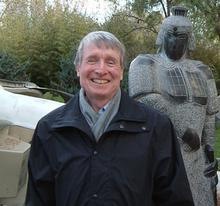
\includegraphics[width=\textwidth]{John_Henry_Holland}
	 	\end{center}
	\end{minipage}
		
	\end{frame}
		
%		
	\begin{frame}
		\frametitle{ 基本思想}
		
		\begin{itemize}
				\item 群体迭代进化。\\它们模拟由个体组成的群体的学习过程,其中每个个体表示给定问题搜索空间中的一个点。进化算法从选定的初始群体出发,通过不断迭代逐步改进当前群体,直至最后搜索到最优解或满意解。
	\end{itemize}
		
	\end{frame}
%		
		
		
		
		
		\begin{frame}\frametitle{总体框架}
			\begin{figure}[htbp]
				\centering
				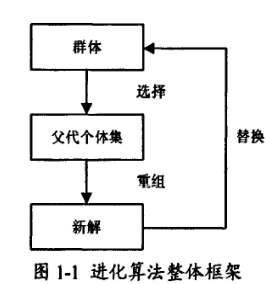
\includegraphics[width=4cm,height=4.5cm]{1}
				
			\end{figure}
			\begin{itemize}
				\item 思想:\dred{群体迭代进化}
				 初始群体 $\rightarrow$迭代逐步改进当前群$\rightarrow$ 搜索到 满意解。 
				\item 重组算子:交叉和变异
				\item 
				\hint{重组算子}用于发现新的候选解 
				\item \hint{替换/选择 算子}则用于确定群体下一步的进化方向 
				
			\end{itemize}
			
		\end{frame}
		
		
		
		
		\begin{frame}
			\frametitle{优缺点}
			
			\begin{itemize}
				\item 优点:
				
				1.从一个群体(多个点)而不是一个点出发进行搜索;\\
				2.易于并行计算;\\
				3.根据适应值选择个体,\hint{采用自然进化机制来求解复杂的优化问题,仅涉及目标函数值的计算,不需要问题的梯度信息;} \\
				4. \hint{一种基于群体的搜索技术} $\rightarrow$ 更强的搜索性能、鲁棒性\\
				5.进化算法在搜索过程中不容易陷入较差的局部最优,即使在所定义的适应度函数是不连续的、非规则的或有噪声的情况下,它们也能以很大的概率找到较好的解;
				
				
			\end{itemize}
			
	 
			
			\begin{itemize}
				\item \dred{缺点:}
				 
			%	1.进化算法只需要用某种编码方式表达问题,然后根据适应值区分个体优劣,因此,编码问题以及合适的进化操作算子的选择需要针对具体问题具体分析,有时难以构造与选择;\\
				
				\dred{1. 应用:迭代次数(适应值评估次数)较多,收敛较慢 }\\
				
				2.理论: 进化算法的理论基础还相当弱 
				
				
			\end{itemize}
			
		\end{frame}
		
		
%		\begin{frame}
%			\frametitle{4.发展与应用现状}
%			
%			\begin{itemize}
%				\item  发展和应用现状:进化算法已在汽车设计、生产调度、电路设计、机器人规划、
%				控制系统设计、电力系统优化设计、天线优化设计、化工过程设计、物流系统设计、
%				时间表安排、任务分配、游戏设计等众多领域得到了十分广泛的应用,并取得了丰硕
%				的成果。
%				
%				
%				
%			\end{itemize}
%			
%		\end{frame}
		
		
	
		
		
		
%		\begin{frame}
%			\frametitle{3.研究现状}
%			\begin{itemize}
%				\item DE的性能要依赖于试验向量产生策略(交叉算子、变异算子)和控制参数(群体规模NP、缩放因子F、交叉控制参数CR),研究人员提出过许多DE的改进版本。\\
%				\textbf{1.}一部分工作集中在改进试验向量产生策略上,例如提出一些新型算子。\\
%				\textbf{2.}另一部分工作是调整DE的控制参数以改善其收敛速度和鲁棒性。
%				\item 将DE与其它搜索算法或搜索技术进行结合。
%				\item 在DE中,如何利用多种群进行搜索也是一个很有意义的研究方向。
%			\end{itemize}
%		\end{frame}
%		
		
		
			
	\section{遗传算法}
	
	\begin{frame}
		\frametitle{简介}
		\begin{itemize}
			\item 自然界中的生物,不断繁殖后代,根据优胜劣汰的原则,不断地进化。进化算法就是借用生物进化的规律,通过繁殖竞争再繁殖再竞争,实现优胜劣汰,一步一步逼近问题的最优解。	
			\item 遗传算法起源于对生物系统所进行的计算机模拟研究。
			\item 其本质是一种高效、并行、全局搜索的方法,能在搜索过程中自动获取和积累有关搜索空间的知识,并自适应地控制搜索过程以求得最佳解。
			\item 遗传算法通过选择、交叉和变异操作来实现个体的更新。遗传算法中,交叉操作对产生新基因起主要作用。
		\end{itemize}
	\end{frame}
	
	
	\begin{frame}
		\frametitle{思想}
		\begin{itemize}
			\item 基本思想:遗传算法中每一条染色体,对应着遗传算法的一个解决方案,一般我们用适应性函数(fitness function)来衡量这个解决方案的优劣。
			\item 所以从一个基因组到其解的适应度形成一个映射。可以把遗传算法的过程看作是一个在多元函数里面求最优解的过程。 可以这样想象,这个多维曲面里面有数不清的“山峰”,而这些山峰所对应的就是局部最优解。
			\item 其中也会有一个“山峰”的海拔最高的,那么这个就是全局最优解。而遗传算法的任务就是尽量爬到最高峰,而不是陷落在一些小山峰。
		\end{itemize}
	\end{frame}
	
	\begin{frame}
		\frametitle{思想}
		\begin{figure}[htbp]
			\centering
			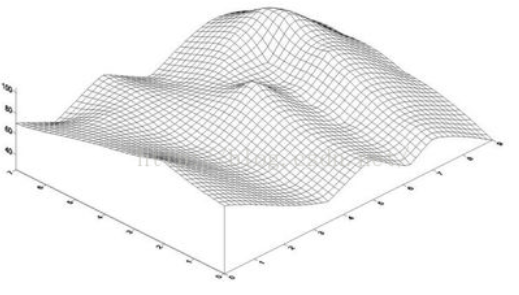
\includegraphics[width=7cm,height=6cm]{figure/3.png}
		\end{figure}
	\end{frame}
	
	\begin{frame}
		\frametitle{一般步骤}
		
			 1. 评估每条染色体所对应个体的适应度。\\
			2. 遵照适应度越高,选择概率越大的原则,从种群中选择两个个体作为父方和母方。\\
			 3. 抽取父母双方的染色体,进行交叉,产生子代。\\
			 4. 对子代的染色体进行变异。\\
			 5. 重复2,3,4步骤,直到新种群的产生。	
	
	\end{frame}
	
	\begin{frame}
		\frametitle{编码方法}
		\begin{itemize}
			\item 二进制编码
			\item 浮点编码法
			\item 符号编码法		
		\end{itemize}
	\end{frame}
	
	\begin{frame}
		\frametitle{二进制编码}
		\begin{itemize}
			\item  一定长度的二进制编码序列,只能表示一定精度的浮点数。
			\item  譬如我们要求解精确到六位小数,区间长度为3, 为了保证精度要求,至少把区间 [-1,2] 分为 $3 * 10^6$ 等份
		\end{itemize}
	\end{frame}
	
	\begin{frame}
		\frametitle{选择算子}
		\begin{itemize}
			\item 轮盘赌选择
			\item 随机竞争选择
			\item 最佳保留选择
			\item 无回放随机选择
			\item 确定式选择
			\item 均匀排序
			\item 最佳保存策略
			\item 随机联赛选择	
		\end{itemize}
	\end{frame}
	
	\begin{frame}
		\frametitle{轮盘赌选择}
		\begin{itemize}
			\item  $F=\sum_{i=1}^Nf_i$
			\item  $P_i=\frac{f_i}{F}$
		\end{itemize}
	\end{frame}
	
	\begin{frame}
		\frametitle{轮盘赌选择}
		\begin{figure}[htbp]
			\centering
			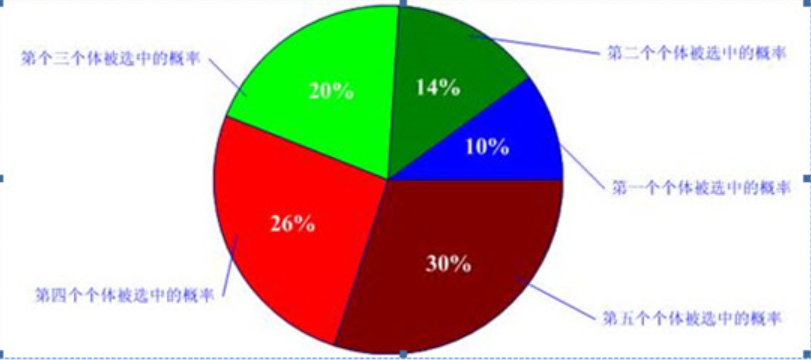
\includegraphics[width=7cm,height=4cm]{figure/4.png}
		\end{figure}
		\end{frame}
	
		\begin{frame}
			\frametitle{随机竞争选择}
			\begin{itemize}
				\item  $ i \in N$   
				\item  $ j \in N$
				\item  $x_k = max\{x_i,x_j\}$
			\end{itemize}
			\end{frame}
		
			\begin{frame}
				\frametitle{染色体交叉}
				\begin{itemize}
					\item 单点交叉
					\item 两点交叉与多点交叉
					\item 均匀交叉 (一致交叉)
					\item 算术交叉	
				\end{itemize}
			\end{frame}
			
			\begin{frame}
				\frametitle{两点交叉}
				
				\begin{figure}[htbp]
					\centering
					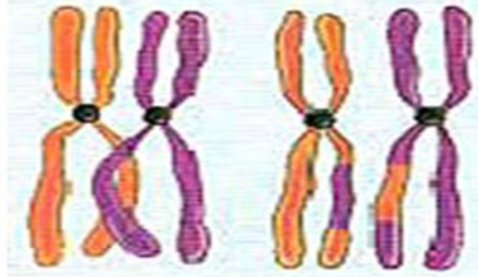
\includegraphics[width=6cm,height=5cm]{figure/5.png}
				\end{figure}
			\end{frame}
			
			\begin{frame}
				\frametitle{基因突变}
				\begin{itemize}
					\item 基本位变异
					\item 两点交叉与多点交叉
					\item 边界变异
					\item 非均匀变异	
					\item 高斯近似变异
				\end{itemize}
			\end{frame}           
			
			
			\begin{frame}
				\frametitle{基本位变异}
				\begin{itemize}
					\item 对个体编码串中以变异概率、随机指定的某一位或某几位仅因座上的值做变异运算。
					\item $101101001011001 \Rightarrow 001101011011001$
				\end{itemize}
			\end{frame}       
			
			\begin{frame}
				\frametitle{边界变异}
				随机的取基因座上的两个对应边界基因值之一去替代原有基因值。特别适用于最优点位于或接近于可行解的边界时的一类问题。
			
			\end{frame}     
				
		\section{差分进化算法(Differential Evolution)}
		
		\begin{frame}
			\frametitle{差分进化算法简介}
			
			\begin{itemize}
				\item 
			差分进化算法(Differential Evolution): 一种基于群体的随机并行搜索算法,它采用变异、交
			叉、替换等算子指导群体进化 
			
			\item 
			在进化过程中,DE保持一个规模为NP的群体(也就是群体中包含NP个个体,每
			个个体为搜索空间中的一个点),并通过迭代的方式改善群体质量 
			
		\end{itemize}
		\end{frame}
		
		\begin{frame}
			\frametitle{DE算法的两方面缺陷}
			
			\begin{itemize}
				\item 种群个体无法继续寻找最优解,停止向全局最优方向进化的现象,即收缩停滞问题
				\item 种群个体失去多样性,陷入局部最优解,即早熟收敛问题
			\end{itemize}
		相应的改进策略主要集中在以下4个方面:控制参数设置、进化策略选择、种群结构以及与其他优化算法混合。
\end{frame}
		
		\begin{frame}
			\frametitle{框架}
			\begin{itemize}
				\item \textbf{Step1 } \hint{初始群体} \\设置当前的代数 $G=0$ 
				从搜索空间S中随机产生  NP个点$\vec{x}_{i, G}, \ldots, \vec{x}_{N P, G}$ 构成初始群体
				\item \textbf{Step2 }\\针对群体中的每个个体$\vec{x}_{i, G}=\left(x_{i, 1, G}, x_{i, 2, G}, \ldots, x_{i, D, G}\right)$,执行变异、修补、交叉、替换4种操作。
			\end{itemize}
		\end{frame}
		
		
		\begin{frame}
			\frametitle{变异}
			\begin{itemize}
				\item \textbf{step2.1变异}: 用DE的变异算子产生一个变异向量$\vec{v}_{i, G}=\left(v_{i, 1, G}, v_{i, 2, G}, \ldots, v_{i, D, G}\right)$ 
		 
			\item 变异算子:
			\quad \hint{$\vec{v}_{i, G}=\vec{x}_{r_1, G}+F \cdot\left(\vec{x}_{r_2, G}-\vec{x}_{r_3, G}\right)$}
			其中, $r_1, r_2, r_3\in \{1, \ldots, N P\}$:随机选择、相互不同,
			 $F$: 缩放因子 
			 
			
			\begin{figure}[h]
				\centering
				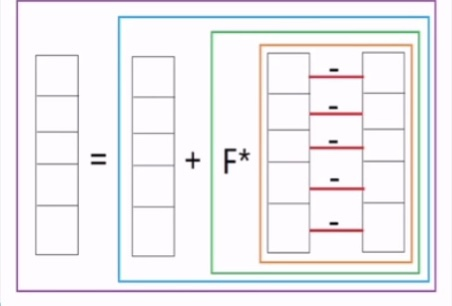
\includegraphics[width=4cm,height=4cm]{变异}	
			\end{figure}
		\end{itemize}
		\end{frame}
		
		
		
		
		\begin{frame}
			\frametitle{修补}
			\begin{itemize}
				\item\textbf{Step2.2修补}:如果变异向量$\vec{v}_{t, G}$为不可行解(落在搜索空间S以外),采用修补算子对$\vec{v}_{t, G}$进行修补,使之成为可行解;
			\end{itemize}
		\end{frame}
		
		
		
		\begin{frame}
			\frametitle{交叉}
			\begin{itemize}
				\item\textbf{Step2.3交叉}:对目标变量$\vec{x}_{t, G}$和变异向量$\vec{v}_{t, G}$,采用交叉算子产生一个试验向量$\vec{u}_{i, G}=\left(u_{i, 1, G}, u_{i, 2, G}, \ldots, u_{i, D, G}\right)$;
				下面看一下二项式交叉。
			\end{itemize}
		\end{frame}
		
		
		
		\begin{frame}
			\begin{figure}[htbp]
				\centering
				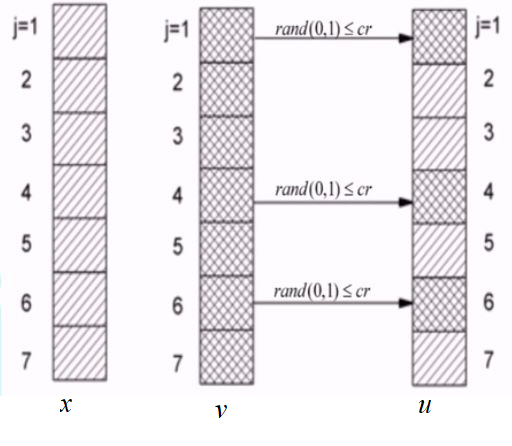
\includegraphics[width=5cm,height=4.5cm]{交叉2}	
			\end{figure}
			$$
			u_{i, j, G}=\left\{\begin{array}{lc}
				v_{i, j, G} & \text { 若 } \operatorname{rand}_{j}(0,1) \leq C R \text { 或 } j=j_{\text {rand }} \\
				x_{i, j, G} & \text {否则  }
			\end{array}\right.
			$$
			
			其中, $j_{\text {rand }}$ 是在区间 $[1, D]$ 中随机选择的整数, $\operatorname{rand}_{j}(0,1)$ 是 0 到 1 之间均匀分布的随机
			数, $C R \in(0,1]$ 称为交叉控制参数。由于 $j_{r a n d}$ 的使用, $\vec{u}_{i, G}$ 不同于 $\vec{x}_{i, G}$ 。
			
			
			
		\end{frame}
		
		
		
		
		
		\begin{frame}
			\frametitle{替换}
			\begin{itemize}
				
				\item\textbf{Step2.4替换}:如果$f\left(\vec{u}_{i, G}\right) \leq f\left(\vec{x}_{i, G}\right)$,令$\vec{x}_{i, G+1}=\vec{u}_{i, G}$;否则,令$\vec{x}_{i, G+1}=\vec{x}_{i, G}$。
			\end{itemize}
		\end{frame}
		
		
		
\begin{frame}
			\frametitle{算法框架}
			\begin{itemize}
					\item 
\textbf{Step\,1初始化种群} :确定需要的参数,在给定搜索区间内随机生成初始的个体

	\item
\textbf{Step\,2.1变异}:变异算子:$n=a+F *(b-c)$ 

	\item \textbf{Step\,2.2交叉} 

	\item
\textbf{Step\,2.3选择(替换)}:
计算目标函数值,比较原始种群以及变异种群中的个体,选出下一代个体  \\

	\item \textbf{Step3\,终止准则判断:}迭代,直到达到设定的最大代数
			\end{itemize}
\end{frame}
		
\begin{frame}
	\frametitle{DE算法示意图}	
	DE在二维搜索空间中的示意图
	\begin{figure}[htbp]
		\centering
		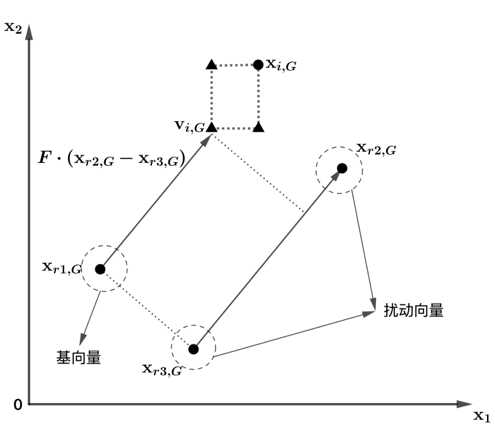
\includegraphics[width=10cm,height=8cm]{DE算法二维搜索空间示意图}
		
	\end{figure}
\end{frame}
\begin{frame}
			\frametitle{示例}
			\begin{itemize}
				\item 应用案例5.10.1   差分进化算法求解无约束二次优化问题   $f(x)=x_{1}^{2}+x_{2}^{2}$
				
			
			\end{itemize}
\end{frame}
		
				\begin{frame}
			\frametitle{练习题}
			\begin{itemize}
				\item 应用   差分进化算法求解无约束二次优化问题     $  f=\sum_{i=1}^{N / 2}\left[\left(x_{2 i}-x_{2 i-1}^{2}\right)^{2}+\left(1-x_{2 i-1}\right)^{2}\right]$
				
				
				%初始点 $x_{0}=(-1.2,1,-1.2,1, \ldots,-1.2,1)^{T} ;$
				最优解  $x^{*}=(1,1, \ldots, 1)^{T} ;$
				最优值  $f^{*}=0$.
				
				
			\end{itemize}
		\end{frame}
		
%	\end{CJK*}
	
	
\end{document}
